\subsection{Caso peggiore metodo moltiplicazione (?)} \label{worst_case_mol}
Come già descritto nella sezione \ref{metodo_mol}, il metodo della moltiplicazione soffre apparentemente di meno criticità. L'unico parametro che possiamo variare per capire se influisce o meno sulle prestazioni è $A$. Come si dimostra negli esempi successivi tuttavia, qualsiasi valore compreso tra $0$ e $1$ è sufficientemente buono, anche se basta distaccarsi di poco dal valore di Knuth\footref{knuth_value} per ottenere risultati sensibilmente differenti.


Utilizzando gli stessi dati di \ref{caso_peggiore_div}, analizziamo le diverse evoluzioni della tabella al variare di $A$. In particolare si pone:
\[
\overbrace{A=(\sqrt{5}-1)/2 = 0,618033...}^{\text{Knuth}} \quad , \quad \overbrace{A=0,848, \quad , \quad A=0,126}^{\text{valori casuali } \in (0;1)}
\]

\begin{figure}[h]
    \begin{center}
    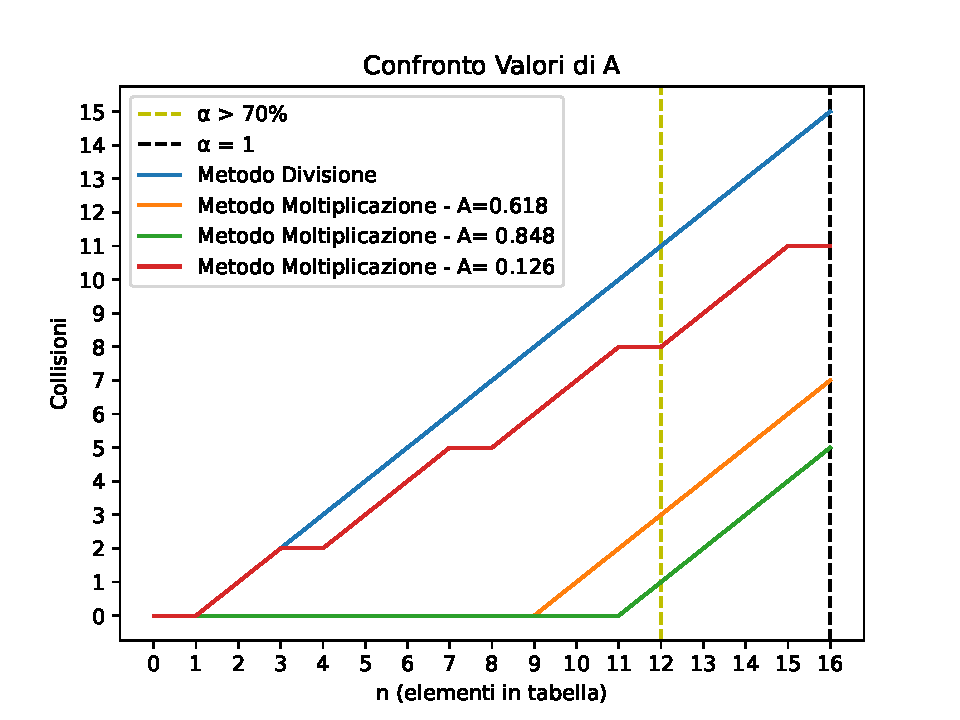
\includegraphics[scale=0.65]{src/img/worstcase_mul.pdf}
    \caption{Evoluzione tabella al variare di $A$}
     \label{fig:worstcase_mul}
    \end{center}
\end{figure}
Il risultato è riportato in Figura \ref{fig:worstcase_mul}. \\ 
Innanzitutto come si nota, tutti e tre i valori utilizzati portano a un risultato migliore rispetto al metodo della divisione in termini di collisioni. \\ 
\'E poi interessante scoprire che ponendo $A = 0.126$ si hanno meno collisioni rispetto al caso $A=(\sqrt{5}-1)/2$. Questo perché il valore di Knuth è \emph{probabilisticamente} migliore, cioè si comporta in generale sempre sufficientemente bene ma in casi specifici ci possono essere alternative migliori. \\
Pertanto complessivamente possiamo dire che non esiste un \emph{caso peggiore} utilizzando il metodo della moltiplicazione, anche se certi valori di $A$ risultano più o meno adatti a seconda dello scenario.